\chapter{Results}
\label{chpt:results}
\section{Introduction}
The previous chapter presented a discussion on the FAP PSO algorithm . This algorithm was developed by modifying the standard PSO algorithm to operate on the FS-FAP. Thus far, no other PSO algorithms have been attempted on the FS-FAP. The only PSO algorithm that has been attempted in the FAP domain was discussed in chapter~\ref{chpt:swarm} and was not relevant to the study in this dissertation, as the PSO was applied to an entirely different FAP variant (MS-FAP). The PSO on the MS-FAP was not relevant because the performance measures and what the algorithms optimise differ.

With the FS-FAP, the main performance measurement is interference and the PSO aims to allocate frequencies in an optimal way to internally produce a frequency plan. On the other hand, the MS-FAP is concerned with the span of frequencies used and the performance measurement is based on the calls dropped. The main purpose of the PSO in the MS-FAP is to minimise the span of frequencies used and keep the number of dropped calls to a minimum.

The previous chapter discussed all the modifications that were made to the standard PSO. The modifications were made to enable PSO to operate on the FAP. Two velocity methods were developed and in addition to the standard global best selection scheme, two additional global best selection schemes were put forward. The algorithm presented was benchmarked against the Siemens instances of the COST 259 benchmark.

This chapter presents the results of applying the FAP PSO algorithm with its different velocity methods as well as different global selection schemes. This is followed by how the different velocity methods affected the PSO performance as well as how the global selection schemes affected the final results.

\section{PSO COST 259 Siemens Results}
The PSO was applied to the benchmarks on the following machine and frameworks:
\begin{itemize}
\item 4 GB RAM
\item Windows 7
\item Intel Quad Core CPU
\item C\# using .Net 4 Framework with Parallel Extensions
\end{itemize}
The FAP PSO was applied to Siemens1, Siemens2, Siemens3 and Siemens4 of the COST 259 benchmark suite. For more information about the nature of the benchmarks, the reader is directed to section \ref{sec:COST259}.

For each benchmark, 12 results are presented. The following changes were made to the FAP PSO to obtain 12 different results one for each variant of the algorithm.
\begin{itemize}
\item The two velocity methods that were developed for the PSO are tested.
\item Each velocity method also used the two different global best mechanisms that were developed.
\end{itemize}
The following values were used for the FAPPSO algorithm regardless of the variant being benchmarked. These values were chosen after a series of trail runs showed that these values produce the best results.
\begin{itemize}
\item The swarm size was set to 20, 50 and 100.
\item Inertia was set to 0.5.
\item Cognitive coefficient was set to 0.4.
\item Social coefficient was set to 0.5.
\item The stopping criteria was set to max iterations 50.
\end{itemize}
The velocity methods and global selection schemes were discussed in the previous chapter. To obtain the best representation for the quality of results produced and performance of the different methods used by the algorithm, the benchmark was executed 20 times for every variant of the algorithm and different population size.

The developed variants of the FAP PSO is compared against the algorithms that were applied the \gls{COST} 259 benchmarks as discussed in chapter 4. Each algorithm against which the FAP PSO is compared against will now be listed. The name this chapter will use to refer to these algorithms are in bold face font. The section the algorithms were discussed in is also be listed. Dynamic Tabu, k-thin FAP, GA

Each section in this chapter presents results on a \gls{COST} 259 benchmark instance and uses the following layout.
\begin{itemize}
        \item A table with results for velocity method 1 and 2. Each table presents the global best selection, population, total interference, average, standard deviation and variance. The average, standard deviation and variance values depicted in this table, were calculated based on the minimum interference achieved across the 20 different algorithm runs.
        \item Within each table the lowest interference obtained is indicated in \textbf{bold}.
        \item A table indicating intrinsic interference information from the generated best plan. The table has the following columns:
            \begin{itemize}
                \item{\textbf{co-channel max}} --- The max co-channel interference generated
                \item{\textbf{co-channel avg}} --- The average co-channel interference generated
                \item{\textbf{co-channel std}} --- The standard deviation of the generated co-channel interference
                \item{\textbf{adj-channel max}} --- The max adjacent-channel interference generated
                \item{\textbf{adj-channel avg}} --- The average adjacent-channel interference generated
                \item{\textbf{adj-channel std}} --- the standard deviation of the generated adjacent interference
                \item{\textbf{TRX max}} --- The max interference generated by a TRX
                \item{\textbf{TRX avg}} --- The avg interference generated by a TRX
                \item{\textbf{TRX std}} --- The standard deviation generated by a TRX
            \end{itemize}
        \item A table indicating the amount of TRX's exceeding a certain interference. The table has the following columns:
            \begin{itemize}
                \item{\textbf{0.01}} --- The amount of TRX pairs whose generated interference exceeds 0.01
                \item{\textbf{0.02} }--- The amount of TRX pairs whose generated interference exceeds 0.02
                \item{\textbf{0.03}} --- The amount of TRX pairs whose generated interference exceeds 0.03
                \item{\textbf{0.04}} --- The amount of TRX pairs whose generated interference exceeds 0.04
                \item{\textbf{0.05}} --- The amount of TRX pairs whose generated interference exceeds 0.05
                \item{\textbf{0.10}} --- The amount of TRX pairs whose generated interference exceeds 0.10
                \item{\textbf{0.15}} --- The amount of TRX pairs whose generated interference exceeds 0.15
                \item{\textbf{0.20}} --- The amount of TRX pairs whose generated interference exceeds 0.20
                \item{\textbf{0.50}} --- The amount of TRX pairs whose generated interference exceeds 0.50
            \end{itemize}
        \item A line graph indicating the progress of the algorithm from iteration 1 to 50 as it obtained the best results for velocity method 1 and method 2.
\end{itemize}

The basis for how the results were produced has now been discussed. Furthermore, a layout for each section has been given. The next section presents the results obtained for the benchmark instance siemens1.
\subsection{Siemens1}
\begin{table}[H]
\centering
	\begin{tabular}{cccccc}
	\toprule
    GBest selection & Population & Interference & Average & Std. Deviation & Variance \\
    \midrule
    Standard & 100 & 100.23 & 103.62 &   9.44 &   4.05\\
    Standard & 50 & 100.90 & 105.69 &  10.44 &   4.19\\
    Standard & 20 & 101.15 & 106.70 &  12.23 &   5.54\\
    GBestFromCells & 20 &  36.41 &  39.60 &   9.09 &   3.18\\
    GBestFromCells & 50 &  \textbf{35.19} &  38.72 &   7.84 &   2.36\\
    GBestFromCells & 100 &  35.27 &  38.82 &   8.80 &   3.52\\
    GBestFromTrxs & 20 & 106.23 & 113.91 &  16.82 &  10.48\\
    GBestFromTrxs & 50 & 107.33 & 114.42 &  16.15 &  10.03\\
    GBestFromTrxs & 100 & 109.80 & 114.94 &  14.61 &   9.70\\
    \midrule
    Dynamic Tabu & --- & N/A & --- & --- & ---\\
    k-Thin SA & --- & 2.20 & --- & --- \\
    GA & --- & 2.96 & --- & --- \\
    \bottomrule
	\end{tabular}
\caption{Siemens1 results with velocity method 1}
\label{tab:siem1m1}
\end{table}
\begin{table}[H]
\centering
	\begin{tabular}{cccccc}
	\toprule
    GBest selection & Population & Interference & Average & Std. Deviation & Variance \\
    \midrule
    Standard & 20 & 378.53 & 784.02 & 794.81 & 23397.43\\
    Standard & 50 & 353.06 & 652.72 & 728.49 & 20411.46\\
    Standard & 100 & 317.16 & 511.48 & 613.45 & 17105.75\\
    GBestFromCells & 20 & 325.69 & 553.86 & 561.71 & 11685.80\\
    GBestFromCells & 50 & 161.25 & 322.53 & 373.15 & 5355.40\\
    GBestFromCells & 100 & 209.01 & 249.04 & 149.56 & 1016.78\\
    GBestFromTrxs & 20 & 193.83 & 577.81 & 1111.87 & 45787.46\\
    GBestFromTrxs & 50 & 149.19 & 347.40 & 885.59 & 30164.26\\
    GBestFromTrxs & 100 & \textbf{142.19} & 244.64 & 417.93 & 7939.47\\
    \midrule
    Dynamic Tabu & --- & \small{N/A} & --- & --- \\
    k-Thin SA & --- & 2.20 & --- & --- \\
    GA & --- & 2.96 & --- & --- \\
    \bottomrule
	\end{tabular}
\caption{Siemens1 results with velocity method 2}
\label{tab:siem1m2}
\end{table}
\begin{table}[H]
\centering
	\begin{tabular}{cccccccccc}
	\toprule
    Algorithm & \multicolumn{3}{c}{co-channel} & \multicolumn{3}{c}{adj-channel} & \multicolumn{3}{c}{TRX}\\
              & max & avg & std
              & max & avg & std
              & max & avg & std\\
    \midrule
    Best FAP PSO & 0.31 & 0.02 & 0.03 & 0.19 & 0.00 & 0.01 & 0.31 & 0.00 & 0.01\\ 
    Dynamic Tabu & \scriptsize{N/A} & \scriptsize{N/A} & \scriptsize{N/A} & \scriptsize{N/A} & \scriptsize{N/A} & \scriptsize{N/A} & \scriptsize{N/A} & \scriptsize{N/A} & \scriptsize{N/A}\\
    k-Thin SA & 0.03 & 0.00 & 0.00 & 0.03 & 0.00 & 0.00 & 0.05 & 0.01 & 0.01\\
    GA & \scriptsize{N/A} & \scriptsize{N/A} &  \scriptsize{N/A} &  \scriptsize{N/A} &  \scriptsize{N/A} &  \scriptsize{N/A} &  \scriptsize{N/A} &  \scriptsize{N/A} & \scriptsize{N/A}\\
    \bottomrule
	\end{tabular}
\caption{co-,adj-channel and TRX interference statistics}
\label{tab:stats-siem1m1}
\end{table}
\begin{table}[H]
\centering
	\begin{tabular}{cccccccccc}
	\toprule
    Algorithm & \multicolumn{9}{c}{TRX pairs exceeding interference}\\
    & 0.01 & 0.02 & 0.03 & 0.04 & 0.05 & 0.10 & 0.15 & 0.20 & 0.50 \\
    \midrule
    Best FAP PSO & 286 & 131 & 98 & 64 & 147 & 31 & 13 & 8 & 0\\
    Dynamic Tabu & \scriptsize{N/A} & \scriptsize{N/A} & \scriptsize{N/A} & \scriptsize{N/A} & \scriptsize{N/A} & \scriptsize{N/A} & \scriptsize{N/A} & \scriptsize{N/A} & \scriptsize{N/A}\\
    k-Thin SA & 33 & 4 & 1 & 0 & 0 & 0 & 0 & 0 & 0 \\
    GA & \scriptsize{N/A} & \scriptsize{N/A} & \scriptsize{N/A} & \scriptsize{N/A} & \scriptsize{N/A} & \scriptsize{N/A} & \scriptsize{N/A} & \scriptsize{N/A} & \scriptsize{N/A}\\
    \bottomrule
	\end{tabular}
\caption{TRX pair interference breakdown}
\label{tab:breakdown-siem1m1}
\end{table}

\subsection{Algorithm run graph for Siemens 1}
\begin{figure}[H]
	\begin{centering}
    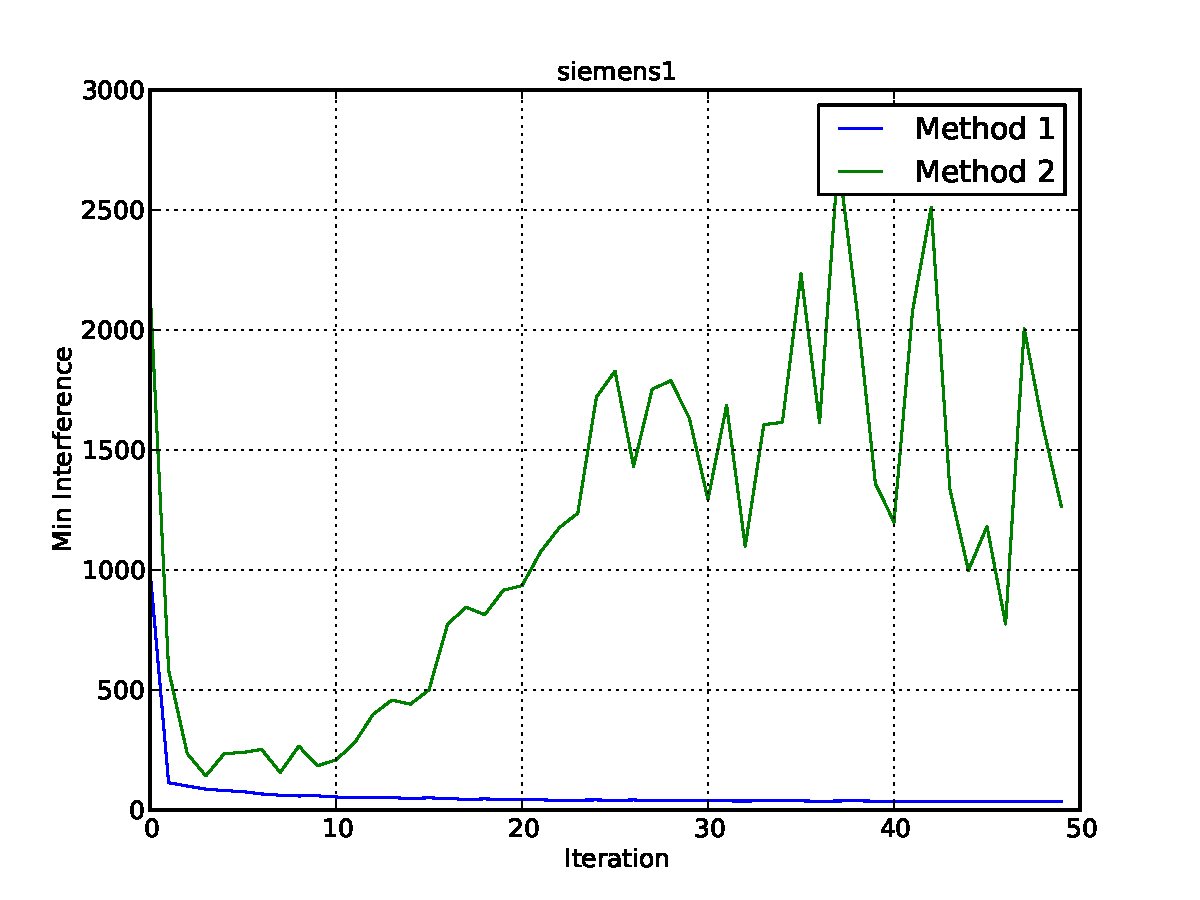
\includegraphics[scale=0.50]{../Implementation/data-cruncher/graph/siemens1.pdf}
	\caption{Algorithm Velocity Method 1 versus Method 2}
	\label{fig:siem1graph}
	\end{centering}
\end{figure}



\subsection{Siemens2}
\begin{table}[H]
\centering
	\begin{tabular}{cccccc}
	\toprule
    GBest selection & Population & Interference & Average & Std. Deviation & Variance \\
    \midrule
    Standard & 20 &  73.32 &  77.65 &   6.20 &   1.43\\
    Standard & 50 &  74.23 &  76.85 &   4.38 &   0.74\\
    Standard & 100 &  74.19 &  76.65 &   3.54 &   0.62\\
    GBestFromCells & 20 &  \textbf{52.63} &  55.55 &   7.93 &   2.33\\
    GBestFromCells & 50 &  53.44 &  55.50 &   5.79 &   1.29\\
    GBestFromCells & 100 &  52.78 &  54.38 &   4.10 &   0.84\\
    GBestFromTrxs & 20 &  77.45 &  81.46 &  12.29 &   5.59\\
    GBestFromTrxs & 50 &  78.00 &  81.04 &   8.08 &   2.51\\
    GBestFromTrxs & 100 &  77.10 &  81.24 &   7.67 &   2.94\\
    \midrule
    Dynamic Tabu & --- & 14.28 & --- & --- & --- \\
    k-Thin SA & --- & 14.27 & --- & ---  & ---\\
    GA & --- & 17.83 & --- & ---  & ---\\
    \bottomrule
	\end{tabular}
\caption{Siemens2 results with velocity method 1}
\label{tab:siem2m1}
\end{table}
\begin{table}[H]
\centering
	\begin{tabular}{cccccc}
	\toprule
    GBest selection & Population & Interference & Average & Std. Deviation & Variance \\
    \midrule
    Standard & 20 & 174.21 & 206.56 &  82.50 & 252.09\\
    Standard & 50 & 161.40 & 207.63 &  90.62 & 315.83\\
    Standard & 100 & 158.31 & 199.62 &  77.74 & 302.17\\
    GBestFromTrxs & 20 & 106.79 & 121.19 &  43.35 &  69.61\\
    GBestFromTrxs & 50 & \textbf{101.03} & 112.28 &  36.08 &  50.07\\
    GBestFromTrxs & 100 & 102.06 & 108.32 &  16.95 &  14.36\\
    GBestFromCells & 20 & 250.15 & 461.26 & 524.44 & 10186.49\\
    GBestFromCells & 50 & 245.19 & 344.08 & 301.00 & 3484.60\\
    GBestFromCells & 100 & 173.36 & 255.28 & 210.97 & 2225.35\\
    \midrule
    Dynamic Tabu & --- & 14.28 & --- & --- & --- \\
    k-Thin SA & --- & 14.27 & --- & --- & --- \\
    GA & --- & 17.83 & --- & --- & --- \\
    \bottomrule
	\end{tabular}
\caption{Siemens2 results with velocity method 2}
\label{tab:siem2m2}
\end{table}
\begin{table}[H]
\centering
	\begin{tabular}{cccccccccc}
	\toprule
    Algorithm & \multicolumn{3}{c}{co-channel} & \multicolumn{3}{c}{adj-channel} & \multicolumn{3}{c}{TRX}\\
              & max & avg & min
              & max & avg & min
              & max & avg & min\\
    \midrule
    Best FAP PSO & 0.23 & 0.01 & 0.02 & 0.02 & 0.00 & 0.00 & 0.23 & 0.12 & 0.12 \\
    Dynamic Tabu & 0.11 & 0.01 & 0.01 & 0.02 & 0.00 & 0.00 & 0.20 & 0.03 & 0.03\\
    k-Thin SA & 0.07 & 0.01 & 0.01 & 0.02 & 0.00 & 0.00 & 0.16 & 0.03 & 0.03\\
    GA & \scriptsize{N/A} & \scriptsize{N/A} & \scriptsize{N/A} & \scriptsize{N/A} & \scriptsize{N/A} & \scriptsize{N/A} & \scriptsize{N/A} & \scriptsize{N/A} & \scriptsize{N/A}\\
    \bottomrule
	\end{tabular}
\caption{co-,adj-channel and TRX interference statistics}
\label{tab:stats-siem2m1}
\end{table}
\begin{table}[H]
\centering
	\begin{tabular}{cccccccccc}
	\toprule
    Algorithm & \multicolumn{9}{c}{TRX pairs exceeding interference}\\
    & 0.01 & 0.02 & 0.03 & 0.04 & 0.05 & 0.10 & 0.15 & 0.20 & 0.50 \\
    \midrule
    Best FAP PSO & 589 & 208 & 1400 & 92 & 193 & 33 & 8 & 3 & 0.00\\
    Dynamic Tabu & 343 & 89 & 24 & 18 & 9 & 1 & 0 & 0 & 0\\
    k-Thin SA & 359 & 71 & 27 & 17 & 13 & 0 & 0 & 0 & 0\\
    GA & \scriptsize{N/A} & \scriptsize{N/A} & \scriptsize{N/A} & \scriptsize{N/A} & \scriptsize{N/A} & \scriptsize{N/A} & \scriptsize{N/A} & \scriptsize{N/A} & \scriptsize{N/A}\\
    \bottomrule
	\end{tabular}
\caption{TRX pair interference breakdown}
\label{tab:breakdown-siem2m1}
\end{table}

\subsection{Algorithm run graph for Siemens 2}
\begin{figure}[H]
	\begin{centering}
    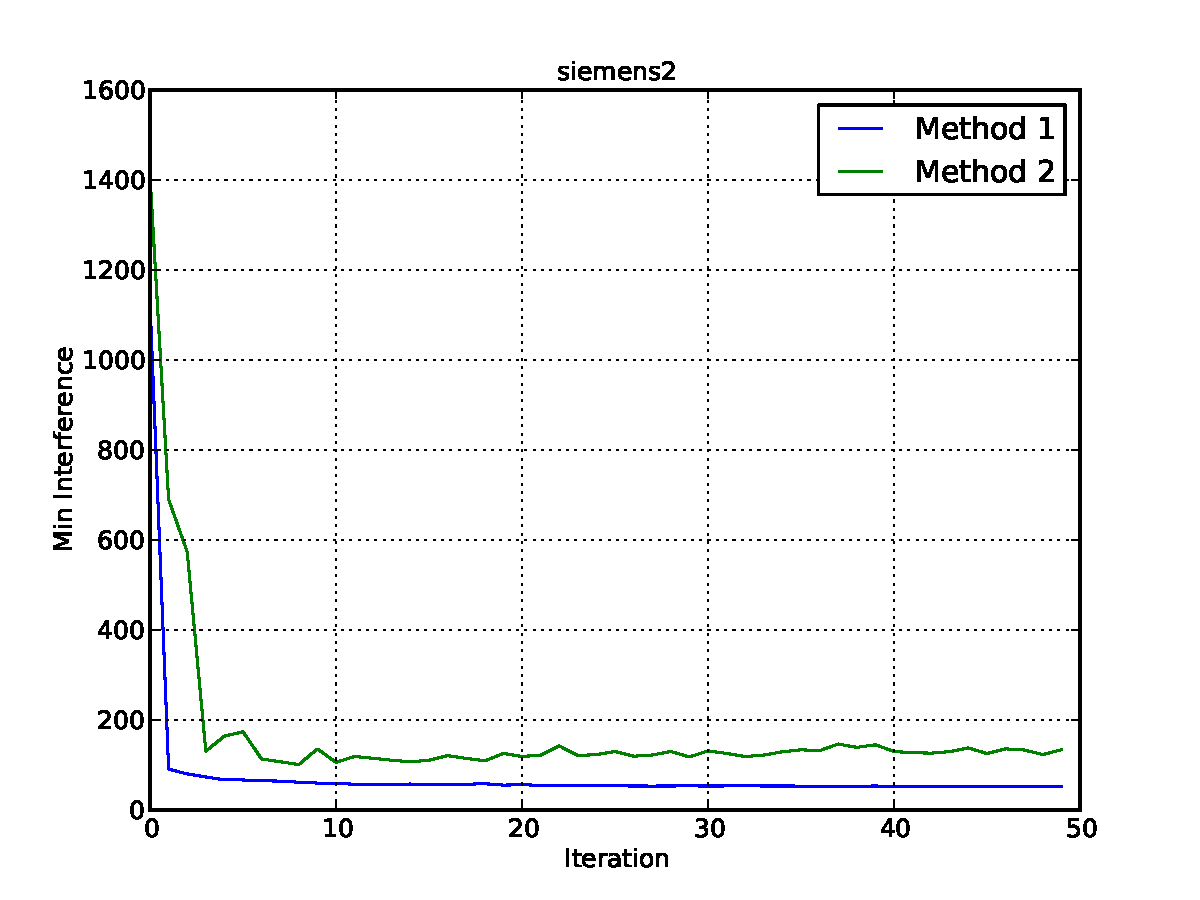
\includegraphics[scale=0.5]{../Implementation/data-cruncher/graph/siemens2.pdf}
	\caption{Algorithm Velocity Method 1 versus Method 2}
	\label{fig:siem2graph}
	\end{centering}
\end{figure}


\subsection{Siemens3}
\begin{table}[H]
\centering
	\begin{tabular}{cccccc}
	\toprule
    GBest selection & Population & Interference & Average & Std. Deviation & Variance \\
    \midrule
    Standard & 20 & 133.47 & 139.18 &  11.77 &   5.54\\
    Standard & 50 & 132.81 & 136.65 &   9.67 &   4.07\\
    Standard & 100 & 131.79 & 135.43 &   8.06 &   3.61\\
    GBestFromCells & 20 &  44.64 &  48.37 &   8.06 &   2.60\\
    GBestFromCells & 50 &  46.50 &  48.79 &   5.08 &   1.12\\
    GBestFromCells & 100 &  45.37 &  48.75 &   7.11 &   2.81\\
    GBestFromTrxs & 20 & 132.93 & 145.69 &  25.55 &  26.12\\
    GBestFromTrxs & 50 & 136.42 & 144.03 &  19.09 &  15.84\\
    GBestFromTrxs & 100 & 136.86 & 145.75 &  17.21 &  16.45\\
    \midrule
    Dynamic Tabu & --- & 1 & --- & --- \\
    k-Thin SA & --- & 2 & --- & --- \\
    GA & --- & 3 & --- & --- \\
    \bottomrule
	\end{tabular}
\caption{Siemens3 results with velocity method 1}
\label{tab:siem3m1}
\end{table}
\begin{table}[H]
\centering
	\begin{tabular}{cccccc}
	\toprule
    GBest selection & Population & Interference & Average & Std. Deviation & Variance \\
    \midrule
    Standard & 20 & 834.88 & 1203.31 & 1037.77 & 43078.83\\
    Standard & 50 & 488.22 & 963.06 & 1439.96 & 90151.59\\
    Standard & 100 & 360.76 & 701.69 & 1064.67 & 62973.79\\
    GBestFromCells & 20 & 413.96 & 571.54 & 535.42 & 11467.16\\
    GBestFromCells & 50 & 269.23 & 392.32 & 319.11 & 4427.39\\
    GBestFromCells & 100 & 221.26 & 315.09 & 203.02 & 2289.75\\
    GBestFromTrxs & 20 & 229.05 & 619.35 & 1365.12 & 74541.80\\
    GBestFromTrxs & 50 & 222.19 & 370.61 & 646.37 & 18165.03\\
    GBestFromTrxs & 100 & 210.01 & 277.58 & 350.43 & 6822.20\\
    \midrule
    Dynamic Tabu & --- & 1 & --- & --- \\
    k-Thin SA & --- & 2 & --- & --- \\
    GA & --- & 3 & --- & --- \\
    \bottomrule
	\end{tabular}
\caption{Siemens3 results with velocity method 2}
\label{tab:siem3m2}
\end{table}
\begin{table}[H]
\centering
	\begin{tabular}{cccccccccc}
	\toprule
    Algorithm & \multicolumn{3}{c}{co-channel} & \multicolumn{3}{c}{adj-channel} & \multicolumn{3}{c}{TRX}\\
              & max & std & max
              & max & std & max
              & max & std & max\\
    \midrule
    Best FAP PSO & 0.22 & 0.01 & 0.02 & 0.14 & 0.00 & 0.01 & 0.22 & 0.00 & 0.00 \\
    Dynamic Tabu & 2 & 3 & 1 & 2 & 3 & 1 & 2 & 3 & 4\\\hline
    k-Thin SA & 2 & 3 & 1 & 2 & 3 & 1 & 2 & 3 & 4\\\hline
    GA & 2 & 3 & 1 & 2 & 3 & 1 & 2 & 3 & 4\\\hline
    \bottomrule
	\end{tabular}
\caption{co-,adj-channel and TRX interference statistics}
\label{tab:stats-siem3m1}
\end{table}
\begin{table}[H]
\centering
	\begin{tabular}{cccccccccc}
	\toprule
    Alg & \multicolumn{9}{c}{TRX pairs exceeding interference}\\
    & 0.01 & 0.02 & 0.03 & 0.04 & 0.05 & 0.10 & 0.15 & 0.20 & 0.50 \\
    \midrule
    Best FAP PSO & 494 & 228 & 150 & 91 & 146 & 27 & 6 & 4 & 0 \\
    Dynamic Tabu & 2 & 3 & 4 & 5 & 6 & 7 & 8 & 9 & 9999\\
    k-Thin SA & 2 & 3 & 4 & 5 & 6 & 7 & 8 & 9 & 12\\
    GA & 2 & 3 & 4 & 5 & 6 & 7 & 8 & 9 & 12\\
    \bottomrule
	\end{tabular}
\caption{TRX pair interference breakdown}
\label{tab:breakdown-siem3m1}
\end{table}

\subsection{Algorithm run graph for Siemens 3}
\begin{figure}[H]
	\begin{centering}
    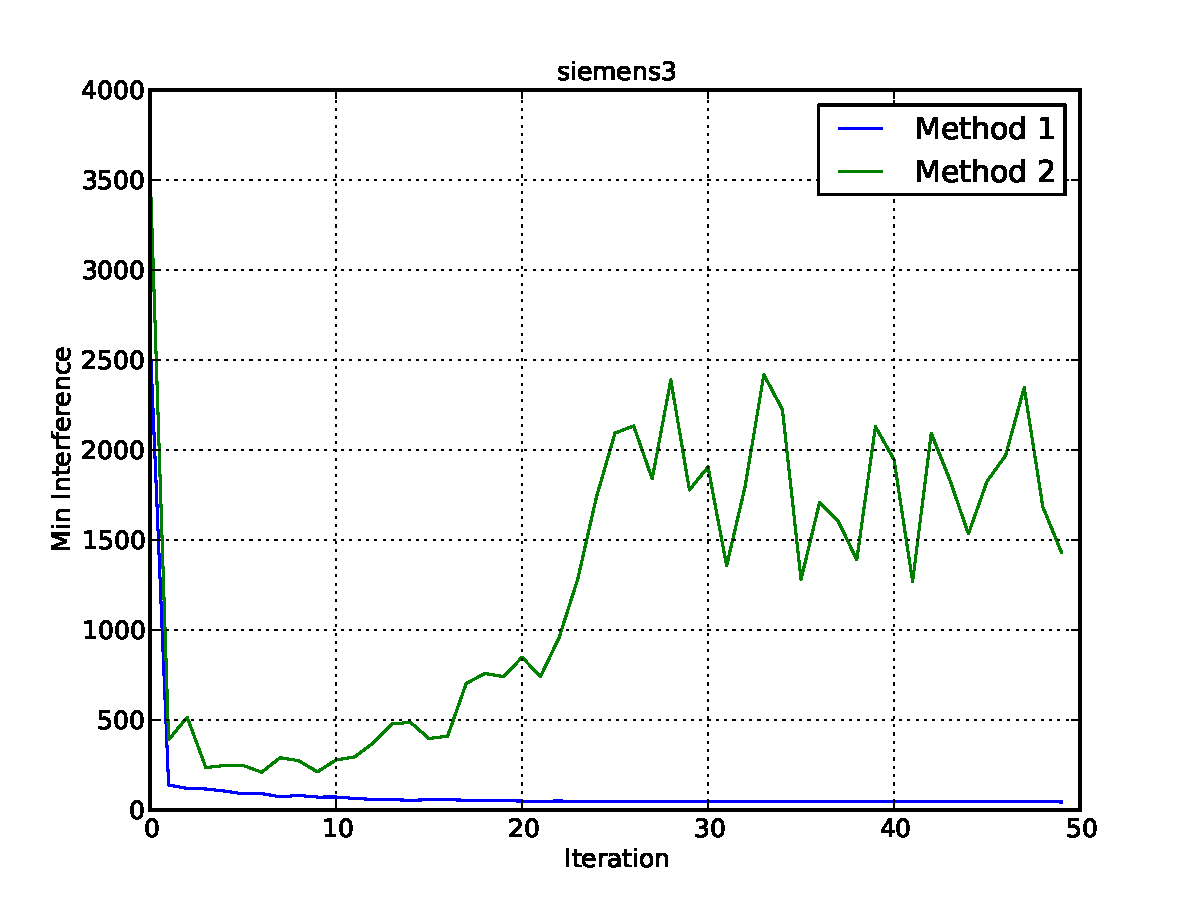
\includegraphics[scale=0.5]{../Implementation/data-cruncher/graph/siemens3.pdf}
	\caption{Algorithm Velocity Method 1 versus Method 2}
	\label{fig:siem3graph}
	\end{centering}
\end{figure}



\subsection{Siemens 4}
\begin{table}[H]
\centering
	\begin{tabular}{cccccc}
	\toprule
    GBest selection & Population & Interference & Average & Std. Deviation & Variance \\
    \midrule
    Standard & 20 & 513.86 & 527.40 &  28.30 &  30.81\\
    Standard & 50 & 507.81 & 521.39 &  25.28 &  29.05\\
    Standard & 100 & 512.97 & 517.03 &   9.02 &  10.17\\
    GBestFromCells & 20 & 284.60 & 291.73 &  26.44 &  26.89\\
    GBestFromCells & 50 & 277.36 & 288.84 &  22.52 &  23.06\\
    GBestFromCells & 100 & 282.36 & 288.14 &  15.41 &  33.94\\
    GBestFromTrxs & 20 & 526.47 & 535.88 &  31.79 &  38.87\\
    GBestFromTrxs & 50 & 518.61 & 533.59 &  35.25 &  56.49\\
    GBestFromTrxs & 100 & 523.24 & 533.67 &  13.59 &  23.07\\
    \midrule
    Dynamic Tabu & --- & 1 & --- & --- \\
    k-Thin SA & --- & 2 & --- & --- \\
    GA & --- & 3 & --- & --- \\
    \bottomrule
	\end{tabular}
\caption{Siemens4 results with velocity method 1}
\label{tab:siem4m1}
\end{table}
\begin{table}[H]
\centering
	\begin{tabular}{cccccc}
	\toprule
    GBest selection & Population & Interference & Average & Std. Deviation & Variance \\
    \midrule
    Standard & 20 & 1482.01 & 2184.35 & 1232.51 & 58426.63\\
    Standard & 50 & 1646.26 & 2058.09 & 987.90 & 44361.28\\
    Standard & 100 & 1746.22 & 2036.60 & 366.09 & 16752.78\\
    GBestFromCells & 20 & 1176.55 & 1572.82 & 1208.47 & 56169.28\\
    GBestFromCells & 50 & 862.67 & 1078.10 & 702.90 & 22457.42\\
    GBestFromCells & 100 & 834.08 & 1007.29 & 286.25 & 10242.22\\
    GBestFromTrxs & 20 & 826.82 & 1761.64 & 2234.28 & 192000.61\\
    GBestFromTrxs & 50 & 942.28 & 1261.93 & 903.42 & 37098.69\\
    GBestFromTrxs & 100 & 844.45 & 1092.90 & 363.64 & 16529.03\\
    \midrule
    Dynamic Tabu & --- & 1 & --- & --- \\
    k-Thin SA & --- & 2 & --- & --- \\
    GA & --- & 3 & --- & --- \\
    \bottomrule
	\end{tabular}
\caption{Siemens4 results with velocity method 2}
\label{tab:siem4m2}
\end{table}
\begin{table}[H]
\centering
	\begin{tabular}{cccccccccc}
	\toprule
    Algorithm & \multicolumn{3}{c}{co-channel} & \multicolumn{3}{c}{adj-channel} & \multicolumn{3}{c}{TRX}\\
              & max & std & max
              & max & std & max
              & max & std & max\\
    \midrule
    Best FAP PSO & 0.57 & 0.01 & 0.03 & 0.08 & 0.00 & 0.00 & 0.57 & 0.00 & 0.00\\
    Dynamic Tabu & 2 & 3 & 1 & 2 & 3 & 1 & 2 & 3 & 4\\\hline
    k-Thin SA & 2 & 3 & 1 & 2 & 3 & 1 & 2 & 3 & 4\\\hline
    GA & 2 & 3 & 1 & 2 & 3 & 1 & 2 & 3 & 4\\\hline
    \bottomrule
	\end{tabular}
\caption{co-,adj-channel and TRX interference statistics}
\label{tab:stats-siem4m1}
\end{table}
\begin{table}[H]
\centering
	\begin{tabular}{cccccccccc}
	\toprule
    Alg & \multicolumn{9}{c}{TRX pairs exceeding interference}\\
    & 0.01 & 0.02 & 0.03 & 0.04 & 0.05 & 0.10 & 0.15 & 0.20 & 0.50 \\
    \midrule
    Best FAP PSO & 1970 & 889 & 452 & 286 & 666 & 253 & 127 & 247 & 5\\
    Tabu & 2 & 3 & 4 & 5 & 6 & 7 & 8 & 9 & 9999\\
    SA & 2 & 3 & 4 & 5 & 6 & 7 & 8 & 9 & 12\\
    GA & 2 & 3 & 4 & 5 & 6 & 7 & 8 & 9  12\\
    \bottomrule
	\end{tabular}
\caption{TRX pair interference breakdown}
\label{tab:breakdown-siem4m1}
\end{table}
\subsection{Algorithm run graph for Siemens 4}
\begin{figure}[H]
	\begin{centering}
    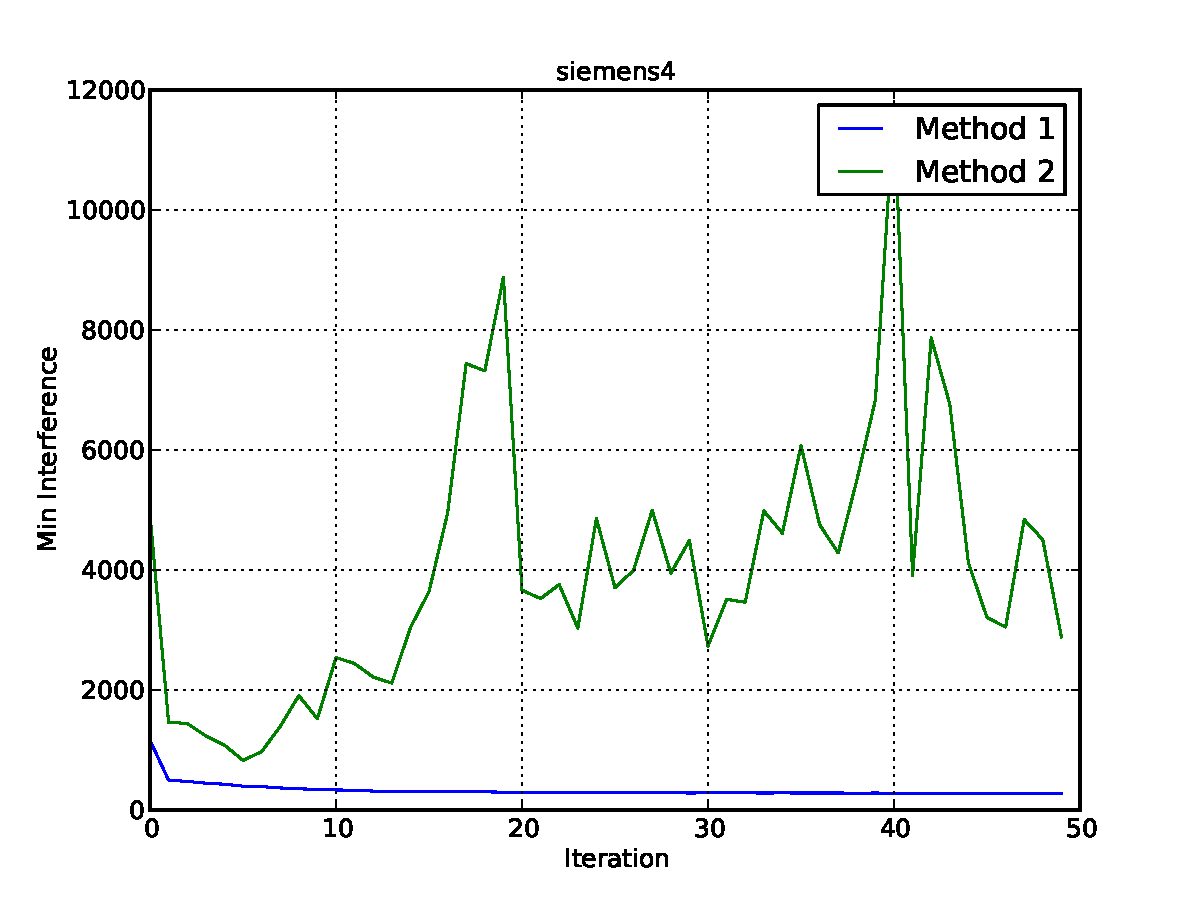
\includegraphics[scale=0.5]{../Implementation/data-cruncher/graph/siemens4.pdf}
	\caption{Algorithm Velocity Method 1 versus Method 2}
	\label{fig:siem4graph}
	\end{centering}
\end{figure}


\subsection{Comparison with best results in COST259}
Below the best results achieved by the FAP PSO is compared to the best results obtained with each Siemens problem as published on the FAP website\cite{FAPWeb}.
\begin{table}[H]
\centering
	\begin{tabular}{| c | c | c | c | c |}
	\hline
	Algorithm & Siemens1 & Siemens2 & Siemens3 & Siemens4 \\ \hline
	FAP PSO & 34.689 & 54.880 & 54.417 & 283.473 \\ \hline
	k-thin FAP & \textbf{2.200} & \textbf{14.271} & \textbf{5.129} & \textbf{77.246} \\ \hline
	Dynamic Tabu Search & --- & 14.275 & 5.186 & 81.876 \\ \hline
	SAG FAP Tool & 2.301 & 14.751 & 5.259 & 80.967 \\ \hline
	\end{tabular}
\caption{FAP PSO results compared to best obtained results}
\label{tab:siem4m2}
\end{table}
\section{The Performance of the PSO}
In this section the effects of the changes made to the FAP PSO algorithm in terms of the results is discussed. First, the effect of the two developed velocity methods in terms of the results is described. 

In section~\ref{sec:diffglobalschemes} the three global schemes that are used by the algorithm are discussed. Finally this section concludes with the effect of a larger population size on solution quality rather than a small population.
\subsection{Velocity Method 1 vs. Method 2}
The FAP PSO algorithm is able to utilise two different velocity methods to move the swarm around in the FAP problem space. The algorithms that implement these two methods were presented in section~\ref{sec:velocityFAP} and section~\ref{sec:velocityFAP2}.

By analysing the results, it becomes abundantly clear that velocity method 1 is by far the superior method for moving in the problem space. In each of the results, when comparing end fitness values produced by algorithm variants that use method 1 one can easily come to the conclusion that method 1 performs better than method 2.

As discussed in chapter~\ref{chpt:psoapplicationFAP}, method 1 uses a stage-based approach when applying the velocity function whereas method 2 applies the velocity function as is without it being broken up. Based on the results, using a stage-based approach to apply the velocity function is far better than applying the velocity equation directly to the transceiver in the plan.

Method 1 works by moving the whole swarm through to each stage before applying the next stage in the velocity equation. Thus after each stage, the whole swarm is at the same phase of the equation which keeps the swarm structured.

With method 2, the whole velocity equation is applied to whatever value is supposed to be operated on. Thus when method 2 moves a particle the frequency plan is moved piece by piece to a destination in the problem space. How method 2 accomplishes this movement was discussed in chapter~\ref{chpt:psoapplicationFAP} section~\ref{sec:velocityFAP2}.

By applying the velocity equation it is difficult to control the algorithm search process. With the FAP PSO control is necessary as there are various constraints that must not only be avoided but also adhered to for the generated plan to be usable. With method 2 adding domain knowledge is difficult, since after the velocity equation has been calculated the particle is very close to being moved to a new position. All that still needs to be done, before a particle is moved, is to apply inertia, which means there is a minor check that can be done to ensure that all the frequency values are within acceptable bounds.

By breaking the velocity equation up into smaller parts (stages) using method 1 the algorithm is able to direct and ensure that the swarm is moving in the general direction of valid frequency allocations.

Also the algorithm is able to embed domain knowledge earlier into the calculation of the velocity and is therefore able to intercept early on movements that will result in invalid frequency allocations at each stage of the velocity equation.

\subsection{Different Global Schemes}
\label{sec:diffglobalschemes}
The previous chapter identified and discussed three global selection schemes. The first global selection scheme uses the standard PSO selection and the particle with the best fitness is the global best. This scheme is called ``Standard GBest''.

As discussed in section~\ref{sec:buildglobalbest}, using the standard gbest selection scheme is not preferable as it can lead to the swarm losing out on good frequency allocations due to overshadowing of frequencies\footnote{Overshadowing is discussed in chapter~\ref{chpt:psoapplicationFAP}}.
Even with overshadowing the standard global scheme does not produce bad results, which seems to indicate that overshadowing of frequency allocations does not impact the frequency plans as significantly as thought initially.

In addition to the standard gbest selection scheme, two other selection schemes were tested. It is incorrect to call these schemes selection schemes of gbest, since they build global best rather than select them.

By far the worst performing scheme is where the global best is built from transceivers. In every benchmark performed where this scheme was paired with a velocity method and population size, the algorithm was simply not able to produce any good solutions. All possible solutions had high interference values, making them undesirable.

The bad performance of the build from transceivers scheme can be attributed to the granularity it uses to build a global best. As outlined in section~\ref{sec:buildglobalbest} the scheme only considers the interference generated by a single frequency allocated to a transceiver. This would have worked well if there were some sort of guarantee that a particular transceiver would only be interfered with by one other transceiver.

In reality and in the Siemens4 benchmarks this is definitely not the case. More often than not, transceivers are interfered with by more than one other transceiver. Thus by only concentrating on a single case-by-case basis of frequencies allocated to transceivers, the scheme is discarding all other possible interferences. 

It might select a frequency at one point as the best, since in that scenario, the interference generated with the only other transceiver that is considered at that point is low. But this particular frequency is too close on the spectrum to another frequency allocated to some other transceiver that also interferes. Due to the algorithm only considering individual cases, this potential interference with the other transceiver will not be noticed by the algorithm and it will go ahead in selecting the frequency as the best for the transceiver.

By analysing the results produced by the various FAP PSO algorithms, it can be concluded that the best global best selection scheme is by far the one in which cells are used to build a global best. With the cell selection scheme, the algorithm does not suffer the pitfall that is the reason for the transceiver gbest building scheme's bad performance.

As discussed the build from cells scheme uses cells to build a gbest, and thus each cell stores the interference that the frequencies allocated to its transceivers generate by interfering with other cells. As a cell interferes with other cells, the interference generated is added to the cell causing the interference.

After the PSO has calculated the fitness of all positions, each cell will contain the interference it personally has caused throughout the network to other cells. A cell with low interference means the frequencies that have been allocated to this particular cell are the best combination that causes the least amount of interference. Therefore, with the build gbest from cells scheme, the algorithm is able to make informed choices when selecting a cell to be included in the global best. 
\subsection{Average and standard deviation}
As can be observed from the results presented the average values the global best achieved across 50 iterations are presented. Also presented is the standard deviation.

By analysing the average and standard deviation it can be concluded that by using velocity method 1, the swarm search process is more directed and focused. The deviation obtained while using velocity method 1 is low meaning that the gbest value of the swarm is near the average value of the gbest obtained across the swarm. Thus by using velocity method 1 the search process of the swarm is more focused and does not explore as much.

On the other hand, with the high deviation and high average, it can be concluded that velocity method 2 lets the swarm explore the problem space a lot more. Even though the search space is explored more, with velocity method 2 the algorithm fails to intensify and converge on a good solution.

\section{Summary}
In this chapter the results produced by the algorithm discussed in chapter~\ref{chpt:psoapplicationFAP} were presented. The FAP PSO algorithm was applied to four COST 259 benchmarks namely Siemens1, Siemens2, Siemens3 and Siemens4. These four benchmarks were discussed in detail in chapter~\ref{chpt:fap}. For each of the benchmarks, 12 different variants of the FAP PSO algorithm were tested. Each variant used a different velocity function, global best selection scheme or population size. The chapter concluded with critical analysis of each of the different algorithms developed in this study to enable the PSO to operate in the FAP space.
